% !TEX root = ../article.tex
% =============================================================================
% 3.5 Desarrollo de la solución
% =============================================================================
% Guía: descripción del modelo, arquitectura o flujo de procesamiento y
% justificación de su elección; solución base de referencia; descripción de
% la implementación (entrenamiento, preentrenados, ajuste fino...); registro
% de experimentos con configuraciones, herramientas, versiones y recursos de
% cómputo. El uso de modelos preentrenados o APIs debe acompañarse de una
% implementación propia y una evaluación que explique su aporte.
%
% Primer avance: propuesta inicial de solución y principales dudas sobre su
% viabilidad.
% =============================================================================

\section{Desarrollo de la solución}\label{sec:development}

% Propuesta inicial para el primer avance: se ajustará tras la asesoría 1.
\subsection{Arquitectura propuesta}\label{sec:architecture}
La propuesta se basa en la U-Net, una red convolucional de codificador y
decodificador con conexiones entre ambos niveles, diseñada para segmentar
imágenes biomédicas con pocos ejemplos anotados \parencite{ronneberger2015}.
Se eligió por tres razones. Primero, sigue siendo la base de los métodos más
sólidos: nnU-Net, que configura automáticamente una U-Net para cada conjunto de
datos, superó a la mayoría de los métodos existentes, incluidas soluciones muy
especializadas, en 23 conjuntos públicos de competencias internacionales de
segmentación biomédica \parencite{isensee2021}. Segundo, en la segmentación pulmonar la
diversidad de los datos pesa más que la arquitectura \parencite{hofmanninger2020},
de modo que conviene invertir el esfuerzo en los datos y en la evaluación más
que en una red novedosa. Tercero, cabe en la GPU disponible en Colab.

La propuesta parte de la solución base y agrega tres mejoras:

\begin{enumerate}
    \item \textbf{Contexto entre cortes (2.5D):} la red recibe como canales de
          entrada el corte que segmenta y sus vecinos inmediatos, y predice la
          máscara del corte central. Así aprovecha la continuidad del pulmón
          entre cortes sin el costo de memoria de una red 3D.
    \item \textbf{Aumentos de datos:} rotaciones, escalados, deformaciones
          elásticas y cambios de intensidad y de ruido, para simular la
          variación entre equipos y pacientes.
    \item \textbf{Datos más diversos:} el entrenamiento combina los estudios de
          rutina de TotalSegmentator con los pulmones con COVID-19
          (Sección~\ref{sec:data}).
\end{enumerate}

La función de pérdida combina Dice y entropía cruzada. Como posprocesamiento,
se conserva la mayor componente conexa de cada pulmón para eliminar
fragmentos aislados, y el volumen de cada pulmón se calcula contando sus
vóxeles y multiplicando por el volumen del vóxel.

\subsection{Solución base}\label{sec:baseline}
La solución base es una U-Net 2D que segmenta cada corte axial por separado,
entrenada con la misma partición y el mismo preprocesamiento que la propuesta,
pero sin contexto entre cortes ni aumentos de datos. Representa la
configuración inicial más simple que todavía es un modelo de Deep Learning
competente. Para medir el aporte de cada mejora, se entrenan además variantes
que agregan una mejora a la vez (estudio de ablación); entre ellas, una
entrenada solo con los casos de COVID-19, para estimar el efecto de la
diversidad de los datos.

TotalSegmentator no es la solución base, sino una referencia publicada: es un
modelo nnU-Net entrenado con más de mil estudios \parencite{wasserthal2023},
que sirve para situar el resultado de Thoraxis frente al estado del arte.

\subsection{Implementación}\label{sec:implementation}
Los modelos se implementan con PyTorch y MONAI, un marco de código abierto
para Deep Learning en salud que incluye transformaciones, redes y métricas
para imagen médica \parencite{cardoso2022}. El repositorio
\texttt{thoraxis-model} se genera con la plantilla ReproPath, que fija la
estructura del proyecto y aporta controles de reproducibilidad, como la
separación por paciente con detección de fugas y el Dice con intervalo de
confianza por \textit{bootstrap}. Los experimentos se
entrenan en Google Colab con GPU, los reentrenamientos automáticos corren en
Kaggle (Sección~\ref{sec:continuous}) y cada corrida se registra en MLflow
(Sección~\ref{sec:experiments}). El modelo elegido se exporta a ONNX, y se
verifica que la versión exportada produce las mismas máscaras que la original
sobre un conjunto de casos de control.

\pendiente{hiperparámetros, número de cortes vecinos, tamaño de las imágenes de
entrada, número de épocas y criterio de parada}

\subsection{Sistema Thoraxis}\label{sec:system}
El sistema tiene tres componentes, cada uno en su repositorio:

\begin{enumerate}
    \item \textbf{Modelo} (\texttt{thoraxis-model}): entrenamiento,
          evaluación y exportación a ONNX.
    \item \textbf{Servicio de inferencia} (\texttt{thoraxis-api}): una API con
          FastAPI que recibe un estudio de TC, aplica el mismo preprocesamiento
          del entrenamiento, ejecuta el modelo con ONNX Runtime, aplica el
          posprocesamiento y devuelve las máscaras y el volumen de cada pulmón
          y, si se pide, el mapa de incertidumbre y la puntuación de confianza
          (Sección~\ref{sec:explainability}). Está instrumentada con
          OpenTelemetry, que mide su rendimiento
          (Sección~\ref{sec:app-monitoring}).
    \item \textbf{Visor web} (\texttt{thoraxis-web}): una aplicación propia en
          Angular que permite cargar un estudio de prueba, recorrer sus cortes
          con la máscara o el mapa de incertidumbre superpuestos y ver los
          volúmenes.
\end{enumerate}

El visor se construye con Angular~22, la versión con soporte activo hasta
junio de 2027 \parencite{angular}, y muestra las imágenes con NiiVue, una
biblioteca de código abierto que visualiza imágenes médicas en el navegador
con WebGL2. NiiVue lee NIfTI directamente, ofrece mapas de color para TC y se
integra en cualquier marco, incluido Angular \parencite{niivue}. La máscara y
el mapa de incertidumbre se superponen al estudio como capas, cada una con su
color y su transparencia. Se descartó levantar un servidor de imágenes médicas
como Orthanc con un visor radiológico completo, porque el prototipo trabaja con
archivos de conjuntos públicos y no necesita recibir estudios de un sistema
hospitalario. Como la aplicación se compila a archivos estáticos, el único
servicio que debe mantenerse en ejecución es la API.

La Figura~\ref{fig:architecture} muestra cómo se relacionan estos componentes
con los datos, el registro de experimentos y los ciclos de retroalimentación
descritos en la Sección~\ref{sec:continuous}.

% Diagrama hecho con Excalidraw: la fuente editable es
% diagrams/thoraxis-architecture.excalidraw, con los logos oficiales incrustados
% (ver diagrams/README.md). Va en una
% página horizontal para que sus etiquetas se lean al imprimir; \afterpage la
% coloca en la página siguiente sin dejar en blanco el resto de la actual.
\afterpage{%
\begin{landscape}
\begin{figure}[p]
    \centering
    \caption{Arquitectura de Thoraxis.}\label{fig:architecture}
    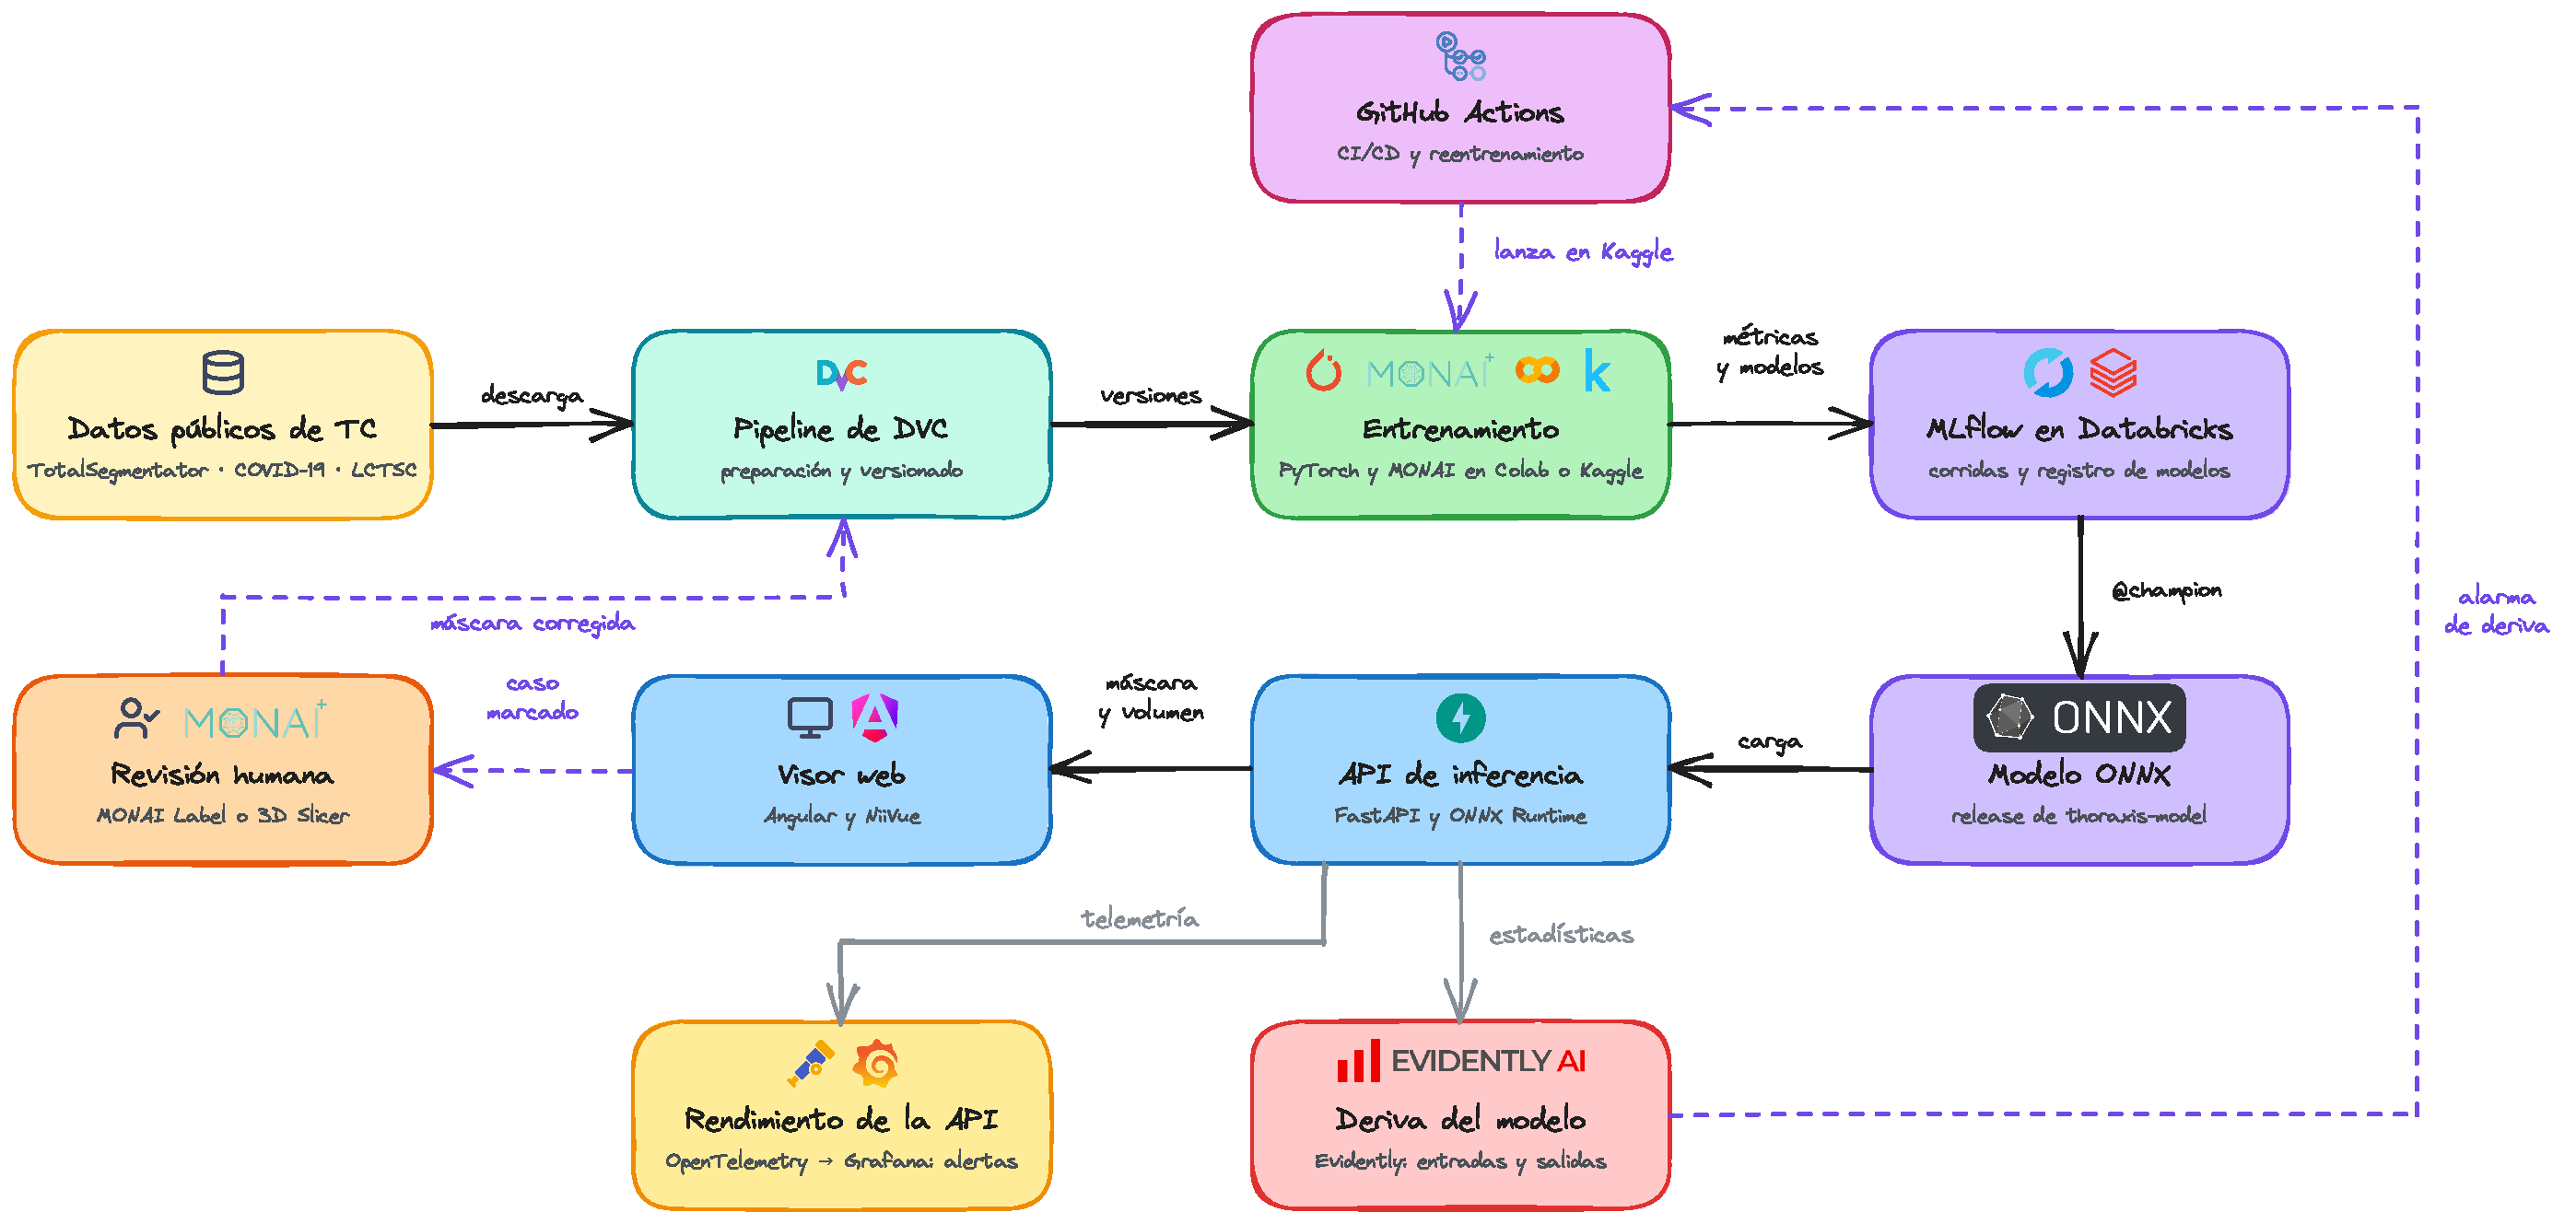
\includegraphics[width=\linewidth]{thoraxis-architecture}
    \articleSource{Elaboración propia con Excalidraw.}
\end{figure}
\end{landscape}}

El prototipo trabaja solo con estudios de los conjuntos públicos y muestra en
todo momento que se trata de una herramienta de investigación. Recibe estudios
en NIfTI, el formato de los datos procesados y de las máscaras. Los estudios
en DICOM, como los de LCTSC, se convierten antes a NIfTI; leerlos directamente
en el navegador, que NiiVue permite convirtiéndolos con dcm2niix compilado a
WebAssembly \parencite{niivuedicom}, queda como extensión futura.

% -----------------------------------------------------------------------------
% Explicabilidad. Afirmaciones verificadas en los resúmenes de cada fuente
% (Crossref, PubMed y Semantic Scholar) el 8 de noviembre de 2026.
% -----------------------------------------------------------------------------
\subsection{Explicabilidad e incertidumbre}\label{sec:explainability}
En imagen médica, la explicabilidad suele asociarse a los mapas de calor que
resaltan las regiones que más influyen en una predicción, como Grad-CAM. La
evidencia, sin embargo, desaconseja usarlos como explicación para el usuario.
En radiografías de tórax, siete de estos métodos, incluido Grad-CAM,
localizaron las patologías significativamente peor que un radiólogo, con la
mayor diferencia en lesiones pequeñas y de forma compleja
\parencite{saporta2022}. En otro estudio, los ocho métodos evaluados fallaron
al menos un criterio de confiabilidad, y varios no cambiaban al aleatorizar los
pesos del modelo, es decir, no reflejaban lo aprendido \parencite{arun2021}. Una
revisión de la explicabilidad en segmentación advierte además que las métricas
actuales para evaluar estos mapas son poco confiables \parencite{gipiskis2024}.

En segmentación resulta más útil mostrar cuánta confianza tiene el modelo en
cada vóxel. La cuantificación de la incertidumbre reduce el efecto de caja
negra de los modelos y hace sus resultados más interpretables y aceptables para
el usuario \parencite{lambert2024}. Las U-Net, en particular, tienden a dar
predicciones demasiado confiadas, tanto cuando aciertan como cuando se
equivocan \parencite{mehrtash2020}. Por eso Thoraxis explica sus segmentaciones
con tres componentes, que se describen con el marco de criterios de
\textcite{vandervelden2022}: todos son explicaciones locales, posteriores al
entrenamiento.

\begin{enumerate}
    \item \textbf{Mapa de incertidumbre por vóxel:} el modelo segmenta varias
          versiones del estudio con aumentos de datos aplicados durante la
          inferencia (\textit{test-time augmentation}), y la variación entre
          esas predicciones se muestra en el visor sobre los cortes. Esta
          técnica estima la incertidumbre mejor que el \textit{dropout} en la
          inferencia y reduce las predicciones erróneas con exceso de
          confianza \parencite{wang2019}; MONAI la implementa
          \parencite{cardoso2022}, por lo que no exige entrenar de nuevo.
    \item \textbf{Puntuación de confianza por caso:} un valor por estudio,
          derivado de la variación del volumen pulmonar entre esas
          predicciones. Los estudios con baja confianza se marcan para la
          revisión humana y la puntuación se envía al monitoreo
          (Sección~\ref{sec:continuous}). Un conjunto de varios modelos
          mejora la calibración de la confianza y permite predecir la calidad
          de la segmentación y detectar estudios distintos a los de
          entrenamiento \parencite{mehrtash2020}; queda como mejora opcional,
          porque multiplica el costo de entrenamiento.
    \item \textbf{Mapas de calor para uso interno:} Seg-Grad-CAM, la extensión
          de Grad-CAM a la segmentación \parencite{vinogradova2020}, se usa
          solo en el análisis de errores del equipo, acompañado de la prueba
          de aleatorizar los pesos del modelo, y no se presenta como
          explicación al usuario.
\end{enumerate}

La incertidumbre explica algo solo si anticipa los errores. Por eso su
evaluación forma parte de la evaluación de la solución
(Sección~\ref{sec:uncertainty-eval}). La inferencia con aumentos multiplica el
tiempo de respuesta por el número de versiones, de modo que el servicio la
ofrece como una opción de la consulta y no en cada predicción.

\subsection{Dudas de viabilidad}\label{sec:feasibility}
Estas son las principales dudas sobre la viabilidad de la propuesta, para
revisar en la primera asesoría:

\begin{enumerate}
    \item \textbf{Cómputo:} las sesiones de Colab duran como máximo 12~horas
          (24 en Pro+) y la GPU depende de la disponibilidad
          \parencite{colabpricing}. ¿Basta para entrenar la propuesta y las
          variantes del estudio de ablación, guardando puntos de control para
          reanudar el entrenamiento?
    \item \textbf{Almacenamiento:} TotalSegmentator ocupa 37,4~GB comprimido.
          ¿Conviene procesar una sola vez un subconjunto de estudios de tórax
          y guardar solo los volúmenes remuestreados?
    \item \textbf{Convenciones de etiquetado:} LCTSC excluye hilios, bronquios
          principales y, en la mayoría de los casos, el tumor
          (Sección~\ref{sec:data-limitations}). ¿Es aceptable fijar el
          criterio de éxito de Dice $\geq 0{,}95$ sobre esas máscaras, o
          conviene reportar también un análisis que separe el efecto de la
          convención?
    \item \textbf{2.5D frente a 3D:} ¿es suficiente el contexto de unos pocos
          cortes vecinos, o se espera comparar con un modelo 3D?
    \item \textbf{Estudios pediátricos:} ¿se incluyen los 291 estudios
          pediátricos de TotalSegmentator, aunque la validación externa sea
          solo con adultos?
    \item \textbf{Licencia del conjunto de COVID-19:} ¿basta con ajustarse a la
          licencia más restrictiva para su uso académico?
    \item \textbf{Entrenamiento continuo:} sin datos reales de pacientes, ¿es
          aceptable demostrarlo con lotes de datos y deriva simulados
          (Sección~\ref{sec:continuous}), y alcanza la cuota semanal gratuita
          de GPU de Kaggle para los reentrenamientos?
    \item \textbf{Compatibilidad de MONAI:} su versión vigente, la 1.6.1,
          declara compatibilidad oficial hasta Python~3.13, y el proyecto usa
          Python~3.14. ¿Conviene fijar Python~3.13 en el repositorio del modelo
          si MONAI no funciona con la versión más reciente?
\end{enumerate}

\subsection{Registro de experimentos y entorno}\label{sec:experiments}
Los experimentos se registran con MLflow \parencite{mlflow}, la plataforma de
código abierto que \textcite{kreuzberger2023} señalan como ejemplo de registro
de modelos y de almacén de metadatos. Cada corrida de entrenamiento guarda sus
parámetros, métricas, artefactos y la versión del código que la produjo, y los
modelos candidatos se versionan en el registro de modelos de MLflow, incluido
el modelo exportado a ONNX. El modelo elegido se publica además como versión
inmutable del repositorio \texttt{thoraxis-model}, que es la que consume el
servicio de inferencia.

El servidor de MLflow es el que ofrece Databricks Free Edition
\parencite{databricksfree}, un espacio de trabajo gratuito para uso no
comercial en el que los tres integrantes comparten los experimentos y el
registro de modelos de Unity Catalog. El entrenamiento corre fuera de
Databricks, en las máquinas del equipo o en Colab, y registra sus resultados
de forma remota con un token de acceso personal; los proyectos en Python se
gestionan con uv y Python~3.14, y MLflow guarda junto a cada modelo el
\texttt{uv.lock} con sus dependencias exactas. Antes de adoptarlo se verificó
desde una máquina local que el registro remoto de corridas y de modelos
funciona en esta edición, porque su documentación no lo especifica.

\pendiente{experimentos y cambios realizados con sus configuraciones
relevantes, versiones de librerías, semillas y recursos de cómputo utilizados}

% -----------------------------------------------------------------------------
% Ciclo de vida, cronograma y MLOps. Las fechas de los hitos salen de la guía
% (sección 4); los principios, de Kreuzberger et al. (2023), lectura del curso.
% Lo que aún no está decidido va como \pendiente.
% -----------------------------------------------------------------------------
\subsection{Ciclo de vida y MLOps}\label{sec:lifecycle}

\subsubsection{Ciclo de vida y cronograma}\label{sec:schedule}
El proyecto sigue un ciclo de vida iterativo, alineado con los tres avances y
la entrega final que fija la guía del proyecto integrador. Cada hito cierra una
iteración con un entregable revisable y una versión del repositorio
(Tabla~\ref{tab:schedule}).

\begin{table}[htbp]
    \centering
    \caption{Fases del ciclo de vida e hitos del proyecto.}\label{tab:schedule}
    \small
    \begin{tabularx}{\textwidth}{>{\raggedright\arraybackslash}p{3.3cm}
                                 >{\raggedright\arraybackslash}p{2.6cm}
                                 >{\raggedright\arraybackslash}X}
        \toprule
        Fase & Hito y fecha & Entregables \\
        \midrule
        Planificación y análisis & Asesoría 1: 6--13 nov 2026 &
            Problema, contexto y evidencia; objetivos; fuente de datos y forma
            de acceso; propuesta inicial y dudas de viabilidad. \\
        Diseño y desarrollo inicial & Asesoría 2: 7--11 dic 2026 &
            Datos preparados o muestra representativa; solución base y
            primeros resultados; diseño, métricas y procedimiento de
            evaluación. \\
        Desarrollo, pruebas e integración & Asesoría 3: 1--5 mar 2027 &
            Prototipo funcional; comparación con la solución base; análisis
            de errores y limitaciones; borrador del informe. \\
        Entrega y sustentación & 20 mar 2027 &
            Informe final, código e instrucciones, datos de prueba o acceso,
            diapositivas y demostración. \\
        \bottomrule
    \end{tabularx}
    \articleSource{Elaboración propia a partir de la guía del proyecto
    integrador.}
\end{table}

\pendiente{tareas por semana dentro de cada fase y responsable de cada una:
preparación de datos, desarrollo, evaluación y documentación}

\subsubsection{Prácticas de MLOps}\label{sec:mlops}
MLOps aplica al aprendizaje automático las prácticas de DevOps para llevar los
modelos a producción de forma automatizada y reproducible.
\textcite{kreuzberger2023} lo sintetizan en nueve principios, que sirven de
guía para el proyecto (Tabla~\ref{tab:mlops}).

\begin{table}[htbp]
    \centering
    \caption{Principios de MLOps y su aplicación en Thoraxis.}\label{tab:mlops}
    \small
    \begin{tabularx}{\textwidth}{>{\raggedright\arraybackslash}p{4.4cm}
                                 >{\raggedright\arraybackslash}X}
        \toprule
        Principio & Práctica en Thoraxis \\
        \midrule
        Automatización de CI/CD & GitHub Actions en cada repositorio: lint,
            pruebas y compilación en cada cambio; versiones con
            release-please. \\
        Orquestación de flujos & Pipeline de DVC con las etapas de
            preparación, entrenamiento, evaluación y exportación, lanzado por
            GitHub Actions en Kaggle. \\
        Reproducibilidad & Plantilla ReproPath en el repositorio del modelo;
            semillas y versiones de librerías fijadas. \\
        Versionado de datos, código y modelo & Código en Git; modelos
            candidatos en el registro de modelos de MLflow; modelo ONNX elegido
            publicado como versión inmutable del repositorio; datos procesados
            versionados con DVC. \\
        Colaboración & Repositorios separados por componente, cambios por pull
            request y revisión entre integrantes. \\
        Entrenamiento y evaluación continuos & Reentrenamiento en Kaggle ante
            datos nuevos o una alarma del monitoreo; cada modelo se evalúa y
            solo se promueve si mejora al vigente
            (Sección~\ref{sec:continuous}). \\
        Seguimiento de metadatos & MLflow Tracking: parámetros, métricas,
            artefactos y versión del código de cada corrida de
            entrenamiento. \\
        Monitoreo continuo & Del modelo: Evidently en el servicio de
            inferencia, para detectar cambios en las estadísticas de entrada y
            de salida. Del aplicativo: OpenTelemetry y Grafana, para la
            latencia, los errores y el uso de recursos de la API. \\
        Ciclos de retroalimentación & Del monitoreo al reentrenamiento, del
            análisis de errores a la preparación de datos y de la revisión
            humana a los datos. \\
        \bottomrule
    \end{tabularx}
    \articleSource{Elaboración propia a partir de
    \textcite{kreuzberger2023}.}
\end{table}

% -----------------------------------------------------------------------------
% Contraste de herramientas. Precios y límites consultados el 8 de noviembre
% de 2026 en las páginas oficiales; revisarlos antes de cada entrega, porque
% cambian sin aviso.
% -----------------------------------------------------------------------------
\subsubsection{Herramientas de MLOps}\label{sec:mlops-tools}
El servidor de MLflow se eligió entre tres opciones: un servidor local,
DagsHub y Databricks. Un servidor local no permite que los tres integrantes
compartan los experimentos, así que la comparación se centró en los dos
servicios gestionados (Tabla~\ref{tab:mlflow-hosting}). Ambos ejecutan MLflow
estándar: el código de entrenamiento es el mismo y solo cambian la dirección
del servidor y las credenciales, de modo que cambiar de servicio más adelante
no obliga a reescribirlo.

\begin{table}[htbp]
    \centering
    \caption{Opciones de alojamiento del servidor de MLflow.}%
    \label{tab:mlflow-hosting}
    \small
    \begin{tabularx}{\textwidth}{>{\raggedright\arraybackslash}p{2.8cm}
                                 >{\raggedright\arraybackslash}X
                                 >{\raggedright\arraybackslash}X
                                 >{\raggedright\arraybackslash}X}
        \toprule
        Criterio & DagsHub (plan gratuito) & Databricks Free Edition &
            Databricks de pago \\
        \midrule
        Costo & Gratis. & Gratis. & Pago por uso en DBU, sin licencia fija;
            prueba de 14 días con hasta 400~USD de crédito. \\
        Equipo de tres & Repositorio público: colaboradores ilimitados.
            Privado: el dueño y dos colaboradores. & Un espacio de trabajo por
            cuenta, compartido con los integrantes invitados. & Sin límite
            relevante. \\
        Experimentos & Repositorio público: ilimitados y visibles para
            cualquiera. Privado: hasta 100. & Sin límite publicado; cuota
            diaria de uso sin cifra publicada. & Según el consumo. \\
        Almacenamiento & 20~GB (la misma página indica también 200~GB). &
            No publicado. & Según el proveedor de nube. \\
        GPU para entrenar & No ofrece cómputo. & Acceso limitado a AI Runtime
            si se verifica la cuenta con LinkedIn. & Clústeres con GPU o AI
            Runtime, con costo por hora (Tabla~\ref{tab:gpu-costs}). \\
        Registro desde PC o Colab & Documentado. & Verificado por el equipo.
            & Documentado. \\
        Uso & No comercial en repositorios privados. & Solo no comercial. &
            Sin restricción. \\
        Riesgos & Experimentos públicos si el repositorio es público. &
            Elimina cuentas inactivas por un período prolongado; sin soporte.
            & Costo variable según el uso. \\
        \bottomrule
    \end{tabularx}
    \articleSource{Elaboración propia a partir de \textcite{dagshubpricing},
    \textcite{databricksfree} y \textcite{databrickspricing}.}
\end{table}

Se eligió Databricks Free Edition porque no limita el número de experimentos,
los mantiene privados al equipo e incluye el registro de modelos de Unity
Catalog; además, Databricks figura entre las plataformas comerciales de MLOps
que revisan \textcite{kreuzberger2023}. Sus riesgos, la cuota diaria y la
posible eliminación de cuentas inactivas, se acotan porque el modelo elegido
se publica en \texttt{thoraxis-model} y el código no depende del servicio.

Para registrar experimentos, el plan de pago de Databricks no aporta nada sobre
el gratuito. La plataforma no cobra una licencia mensual, sino el cómputo
consumido: en AWS, plan Premium y región US East, el cómputo interactivo
\textit{serverless} cuesta 0{,}75~USD por DBU y los trabajos
\textit{serverless}, 0{,}35~USD por DBU, con la infraestructura incluida
\parencite{databrickspricing, databricksjobs}. MLflow gestionado viene incluido
en ese cómputo y no tiene una tarifa propia publicada. El plan Team de DagsHub
cuesta 99~USD por usuario al mes con pago anual y 119~USD con pago mensual
\parencite{dagshubpricing}, es decir, entre 297 y 357~USD al mes para tres
integrantes. Por eso el registro de experimentos se mantiene en el plan
gratuito.

El entrenamiento con GPU es otro asunto. El equipo entrena en Google Colab,
que cobra por unidades de cómputo: el plan Pro cuesta 9{,}99~USD al mes con
100 unidades y el Pro+, 49{,}99~USD con 600; las unidades vencen a los 90
días, y Pro+ mantiene la ejecución hasta 24~horas con el navegador cerrado
\parencite{colabpricing}. Google no publica cuántas unidades por hora consume
cada GPU, y las GPU disponibles dependen de la demanda. Databricks ofrece dos
alternativas de pago (Tabla~\ref{tab:gpu-costs}). En los clústeres clásicos, la
máquina con GPU se paga a AWS y los DBU a Databricks, lo que exige una cuenta
propia de AWS \parencite{databrickscalculator, awsec2}. AI Runtime, en vista
previa, cobra un precio único por hora de GPU con la infraestructura incluida
\parencite{databricksairuntime}. Free Edition, por su parte, da acceso limitado
a AI Runtime si se verifica la cuenta con LinkedIn, sin publicar cuántas horas
\parencite{databricksfree}.

\begin{table}[htbp]
    \centering
    \caption{Costo del entrenamiento con GPU en Databricks.}%
    \label{tab:gpu-costs}
    \small
    \begin{tabularx}{\textwidth}{>{\raggedright\arraybackslash}X
                                 >{\raggedright\arraybackslash}p{2.6cm}
                                 >{\raggedright\arraybackslash}p{2.2cm}
                                 >{\raggedright\arraybackslash}p{2.2cm}}
        \toprule
        Opción & GPU & USD por hora & 100~horas al mes \\
        \midrule
        Clásico, como trabajo & T4 (16~GB) & 0{,}63 & 63~USD \\
        Clásico, como trabajo & A10G (24~GB) & 1{,}21 & 121~USD \\
        Clásico, en notebook interactivo & A10G (24~GB) & 1{,}75 & 175~USD \\
        AI Runtime (vista previa) & A10 (24~GB) & 2{,}50 & 250~USD \\
        AI Runtime (vista previa) & H100 (80~GB) & 7{,}00 & 700~USD \\
        AI Runtime en Free Edition & Sin publicar & Gratis, con acceso
            limitado & Sin publicar \\
        \bottomrule
    \end{tabularx}
    \articleSource{Elaboración propia a partir de
    \textcite{databrickscalculator}, \textcite{awsec2},
    \textcite{databricksairuntime} y \textcite{databricksfree}. AWS, plan
    Premium, región US East; el costo clásico suma la instancia de AWS
    (\texttt{g4dn.xlarge} y \texttt{g5.xlarge}) y los DBU de Databricks.}
\end{table}

Para el desarrollo se mantiene Colab para entrenar y Databricks Free Edition
para registrar los experimentos. Pagar Databricks se justificaría solo si
Colab no alcanza, por ejemplo con entrenamientos de más de 24~horas o si se
necesita una GPU garantizada; en ese caso, AI Runtime evita administrar una
cuenta de AWS, y la prueba gratuita de 14 días incluye hasta 400~USD de crédito
\parencite{databrickstrial}.
\pendiente{horas de GPU estimadas por mes y acceso a AI Runtime obtenido con la
verificación de Free Edition}

MLflow sobre Databricks cubre solo una parte de los principios de la
Tabla~\ref{tab:mlops}. La Tabla~\ref{tab:mlflow-coverage} contrasta qué
resuelve y qué queda a cargo de otras herramientas.

\begin{table}[htbp]
    \centering
    \caption{Cobertura de MLflow sobre Databricks frente a los principios de
    MLOps.}\label{tab:mlflow-coverage}
    \small
    \begin{tabularx}{\textwidth}{>{\raggedright\arraybackslash}p{4.4cm}
                                 >{\raggedright\arraybackslash}p{1.7cm}
                                 >{\raggedright\arraybackslash}X}
        \toprule
        Principio & Cobertura & Detalle \\
        \midrule
        Seguimiento de metadatos & Completa & MLflow Tracking registra
            parámetros, métricas, artefactos y el commit de cada corrida. \\
        Versionado del modelo & Completa & El registro de Unity Catalog
            versiona cada modelo; un alias como \texttt{@champion} marca el
            elegido. \\
        Versionado de datos & Parcial & \texttt{mlflow.log\_input} guarda una
            huella del conjunto usado en cada corrida, sin copiar los datos. \\
        Reproducibilidad & Parcial & Cada modelo registrado guarda el
            \texttt{uv.lock}, los parámetros y el commit; las semillas y
            ReproPath dependen del código. \\
        Colaboración & Parcial & Espacio de trabajo compartido por los tres
            integrantes; la revisión de código sigue en GitHub. \\
        Automatización de CI/CD & Ninguna & GitHub Actions; un flujo puede
            consultar el registro para saber qué versión publicar. \\
        Orquestación de flujos & Ninguna & DVC y GitHub Actions; Databricks
            ofrece trabajos programados, pero el entrenamiento corre en Colab y
            Kaggle. \\
        Monitoreo continuo & Ninguna & Evidently, OpenTelemetry y Grafana en
            \texttt{thoraxis-api}; el monitoreo de Databricks está pensado para
            modelos servidos en la propia plataforma. \\
        Entrenamiento continuo y retroalimentación & Parcial & Los alias del
            registro distinguen el modelo candidato del vigente; el
            reentrenamiento corre en Kaggle y lo disparan GitHub Actions y
            Evidently. \\
        \bottomrule
    \end{tabularx}
    \articleSource{Elaboración propia a partir de \textcite{mlflow} y
    \textcite{kreuzberger2023}.}
\end{table}

% -----------------------------------------------------------------------------
% Entrenamiento continuo y retroalimentación (principios de Kreuzberger et al.,
% 2023). Herramientas y cuotas verificadas el 8 de noviembre de 2026.
% -----------------------------------------------------------------------------
\subsubsection{Entrenamiento continuo y retroalimentación}\label{sec:continuous}
Según \textcite{kreuzberger2023}, el entrenamiento continuo reentrena el modelo
cuando hay datos nuevos, se apoya en el monitoreo, en un ciclo de
retroalimentación y en un pipeline automatizado, y siempre incluye una
evaluación del cambio en la calidad del modelo. Los ciclos de
retroalimentación, por su parte, llevan lo aprendido en la evaluación de
vuelta al desarrollo, y lo observado en el monitoreo, al disparador del
reentrenamiento.

\paragraph{Dónde se reentrena.}
Colab no ofrece una forma gratuita de programar ejecuciones: la programación es
una función de Colab Enterprise, un servicio de pago de Google Cloud
\parencite{colabschedule}. GitHub Actions ofrece máquinas con GPU T4 a
0,052~USD por minuto, pero solo para organizaciones con planes de pago
\parencite{githubrunners}. Por eso el reentrenamiento automático corre en
Kaggle Notebooks, que ofrece gratis una GPU P100 o dos T4, con sesiones de
hasta 12~horas y una cuota semanal, y permite programar ejecuciones o
dispararlas cuando se actualiza un conjunto de datos \parencite{kagglenotebooks}.
Su interfaz de línea de comandos, además, lanza un notebook con GPU desde un
flujo de GitHub Actions \parencite{kagglecli}. Colab se mantiene para la
experimentación interactiva.

\paragraph{Flujo de reentrenamiento.}
\begin{enumerate}
    \item \textbf{Disparo:} una versión nueva de los datos procesados, que se
          versionan con DVC \parencite{dvc}, o una alarma del monitoreo.
    \item \textbf{Ejecución:} GitHub Actions lanza en Kaggle el pipeline de
          DVC, con las etapas de preparación, entrenamiento, evaluación y
          exportación, y la corrida queda registrada en MLflow.
    \item \textbf{Evaluación:} el modelo nuevo se evalúa en la prueba interna
          fija y en LCTSC, y se registra en Unity Catalog con el alias
          \texttt{@challenger} \parencite{databricksaliases}.
    \item \textbf{Promoción:} un control en GitHub Actions lo compara con el
          modelo vigente, identificado con el alias \texttt{@champion}. Solo
          si lo supera y cumple el criterio de éxito
          (Sección~\ref{sec:expected-outcome}) recibe ese alias, y su versión
          ONNX se publica en \texttt{thoraxis-model} tras la aprobación de un
          integrante.
\end{enumerate}

\paragraph{Ciclos de retroalimentación.}
Thoraxis implementa tres:

\begin{itemize}
    \item \textbf{Del monitoreo al reentrenamiento:} el servicio de inferencia
          registra con Evidently solo estadísticas de cada estudio, nunca las
          imágenes: a la entrada, el espaciado, el espesor de corte y los
          percentiles de intensidad; a la salida, el volumen de cada pulmón,
          la relación entre ambos, el número de fragmentos y la puntuación de
          confianza. Evidently
          convierte la comparación con los datos de referencia en pruebas que
          pasan o fallan \parencite{evidently}; si fallan, GitHub Actions
          dispara el reentrenamiento.
    \item \textbf{De la evaluación al desarrollo:} los casos de error del
          análisis (Sección~\ref{sec:errors}) vuelven a la preparación de
          datos, por ejemplo para incorporar más pulmones con patología.
    \item \textbf{De la revisión humana a los datos:} en el visor, un revisor
          marca una segmentación incorrecta, o el sistema marca una de baja
          confianza (Sección~\ref{sec:explainability}); el caso se corrige en
          MONAI
          Label, un marco de anotación interactiva asistida por IA para
          imágenes médicas 3D \parencite{diazpinto2024}, y la máscara
          corregida entra en una versión nueva de los datos, que dispara el
          reentrenamiento. La última versión publicada de MONAI Label es de
          octubre de 2023, aunque su repositorio sigue recibiendo cambios; si
          no funciona con el entorno del proyecto, las correcciones se harán a
          mano en 3D Slicer.
\end{itemize}

El proyecto no recibe datos de pacientes, así que no llegarán datos nuevos por
sí solos. Para demostrar los ciclos se simulan: una parte de los estudios de
TotalSegmentator se reserva como datos futuros que llegan por lotes, y la
deriva se simula con estudios de otra fuente o con cortes más gruesos. Los
resultados se presentarán como una demostración del mecanismo, no como un
sistema en operación. La Figura~\ref{fig:architecture} resume el flujo
completo, de los datos al visor web, junto con los tres ciclos de
retroalimentación.

% -----------------------------------------------------------------------------
% Monitoreo del aplicativo. Límites del plan gratuito de Grafana Cloud y versión
% de la instrumentación de FastAPI verificados el 8 de noviembre de 2026.
% -----------------------------------------------------------------------------
\subsubsection{Monitoreo del aplicativo}\label{sec:app-monitoring}
Evidently vigila el modelo, pero no si el servicio responde a tiempo. Para eso
la API se instrumenta con OpenTelemetry, un marco de código abierto para
generar, recolectar y exportar trazas, métricas y registros sin depender de un
proveedor. OpenTelemetry no guarda ni muestra los datos: deja esas tareas a
otras herramientas \parencite{opentelemetry}. Su instrumentación para FastAPI
mide cada petición de forma automática, y su versión 0.66b2, todavía en
fase beta, declara compatibilidad con Python~3.14 \parencite{otelfastapi}. La
API emite tres tipos de datos:

\begin{itemize}
    \item \textbf{Métricas:} peticiones por minuto, tasa de errores y latencia
          de cada endpoint, más métricas propias del proyecto: el tiempo de
          preprocesamiento, el de inferencia con ONNX Runtime, el de la
          inferencia con aumentos para el mapa de incertidumbre y la memoria
          del proceso.
    \item \textbf{Trazas:} cada consulta se divide en tramos (carga del
          estudio, preprocesamiento, inferencia y posprocesamiento), lo que
          permite ubicar la etapa lenta.
    \item \textbf{Registros:} los errores, con el identificador de su traza.
          Igual que en Evidently, solo se registran metadatos, nunca las
          imágenes.
\end{itemize}

Los datos se envían a Grafana Cloud, que recibe OpenTelemetry directamente. Su
plan gratuito incluye 10\,000 series activas de métricas, 50~GB de registros y
50~GB de trazas al mes, con 14~días de retención, y hasta tres usuarios
activos, el tamaño del equipo \parencite{grafanapricing}. En Grafana se arma un
panel con el rendimiento de la API y alertas que avisan al equipo cuando la
latencia o la tasa de errores superan un umbral. A diferencia de las pruebas de
Evidently, estas alertas no disparan el reentrenamiento, porque un problema de
rendimiento no se resuelve reentrenando el modelo. Las mismas mediciones
alimentan la evaluación del tiempo de respuesta y de los recursos
(Sección~\ref{sec:resources}); como la retención es de 14~días, se exportan al
terminar cada evaluación. El visor web no se instrumenta, porque el costo
está en la API.

\subsection{Material técnico y reproducibilidad}\label{sec:repositories}
El código del proyecto se organiza en cuatro repositorios:

\begin{itemize}
    \item \textbf{Modelo:} entrenamiento, evaluación y exportación.
          \url{https://github.com/ahincho/thoraxis-model}
    \item \textbf{API:} servicio de inferencia.
          \url{https://github.com/ahincho/thoraxis-api}
    \item \textbf{Web:} visor de cortes con la máscara de segmentación.
          \url{https://github.com/ahincho/thoraxis-web}
    \item \textbf{Informe:} este documento.
          \url{https://github.com/ahincho/thoraxis-article}
\end{itemize}

\pendiente{instrucciones para reproducir la evaluación y acceso a los datos de
prueba}
